%!TEX root = ../thesis_a4.tex

\chapter{Applications}
\label{chap:applicatoins}

\section{Introduction}
\label{sec:applications_introduction}

The research work presented in this thesis has several applications. A number of these applications have already been identified and described in~\secref{sec:motivation}. While some applications such as \gls{raga}-based music retrieval and music discovery are relevant largely in the context of large audio collections, there are several applications that can be developed on the scale of the corpora compiled in the CompMusic project. In this chapter we present some concrete examples of such applications that have already incorporated parts of the outcome of our work. We provide a brief overview of Dunya, a collection of music corpora and software tools developed during the project (\chapref{chap:corpus_music_corpora_and_datasets}) and, \Gls{saraga} and \Gls{riyaz}, the mobile applications developed within the technology transfer project, \gls{camut}. In addition, we present three Web demos that showcase parts of the outcomes of our computational methods. We also briefly present one of our recent study that perform musicologically motivated exploration of melodic structures in \gls{iam}. It acts as an example of how our methods can facilitate investigations in computational musicology.\TODO{include this last sentence only if you provide enough description}

\section{Dunya}
\label{sec:applications_dunya}

Dunya\footnote{\url{http://dunya.compmusic.upf.edu/}} comprises the music corpora and the software tools that have been developed as part of the CompMusic project. It includes data for five music traditions - Hindustani, Carnatic, Turkish Makam music, Jingju and Andalusian music. By providing access to the gathered and the generated data in the project, Dunya aims to facilitate study and exploration of relevant aspects of different music repertoires. CompMusic corpora mainly comprise audio recordings and complementary information that describes those recordings. This complementary information can be in the form of the relevant metadata, melody, rhythm and structural descriptors extracted using computational analyses and, wherever relevant, music scores. The metadata for each recording is aggregated from multiple data sources; MusicBrainz, for the editorial metadata and, Wikipedia, for artists' biographies\footnote{An~example~of~a~biography,~\url{https://en.wikipedia.org/wiki/T._M._Krishna}} and related information. For a detailed description of Dunya we refer to~\cite{dunya_porter}.

To extract the music descriptors mentioned above Dunya uses \gls{essentia} and a set of software packages developed for specific music traditions. Our work on tonic identification is already integrated in to \gls{essentia}, and is thus available in Dunya. Implementations of our other methods for pattern discovery and \gls{raga} recognition will also be integrated into \gls{essentia}. 

There are two modes in which Dunya provides access to the data mentioned above; a Web-based interface, and a restful \acrshort{api}. The Web-based GUI\footnote{\url{http://dunya.compmusic.upf.edu/}} is mainly meant to browse through the music corpora, listen to the music recordings, and visualize the extracted music descriptors time-synchronized with the music. In a way it also provides a medium for enhanced music listening. In addition, for every recording the associated metadata is also shown, which provides the surrounding context to better appreciate the music performance. A screenshot of the recording page for a music piece\footnote{\url{http://dunya.compmusic.upf.edu/hindustani/recording/72df913b-ac52-4798-990d-72e04a64bd8c/raga-ragesri}}\footnote{\url{http://musicbrainz.org/recording/72df913b-ac52-4798-990d-72e04a64bd8c}} in Hindustani music is shown in~\figref{fig:dunya_recording}. We see that there are three main panes, the metadata pane towards top-left, rhythm pane at the top and melody pane at the bottom. The metadata pane displays the editorial and the automatically generated metadata. In this pane, the main description of the melodic aspects of performance is given by the tonic and the \gls{raga} label, indicated by the arrows numbered 1~and~5, respectively. The melody pane at the bottom displays a coarse timbral representation on top which the extracted predominant pitch contour is shown (indicated by arrow-3).  In the same pane, the solid horizontal line (indicated by arrow-2) marks the tonic frequency of the recording. This frequency corresponds to the base \gls{svara} Sa in the performance and acts as a reference to better interpret the pitch intervals (or values) in the continuous pitch contour. The second octave of the tonic frequency is also indicated by a dashed horizontal line. Along with the predominant pitch contour its histogram is also shown (arrow-4), which summarizes the overall pitch material used in the entire performance. 

\begin{sidewaysfigure}
	\begin{center}
		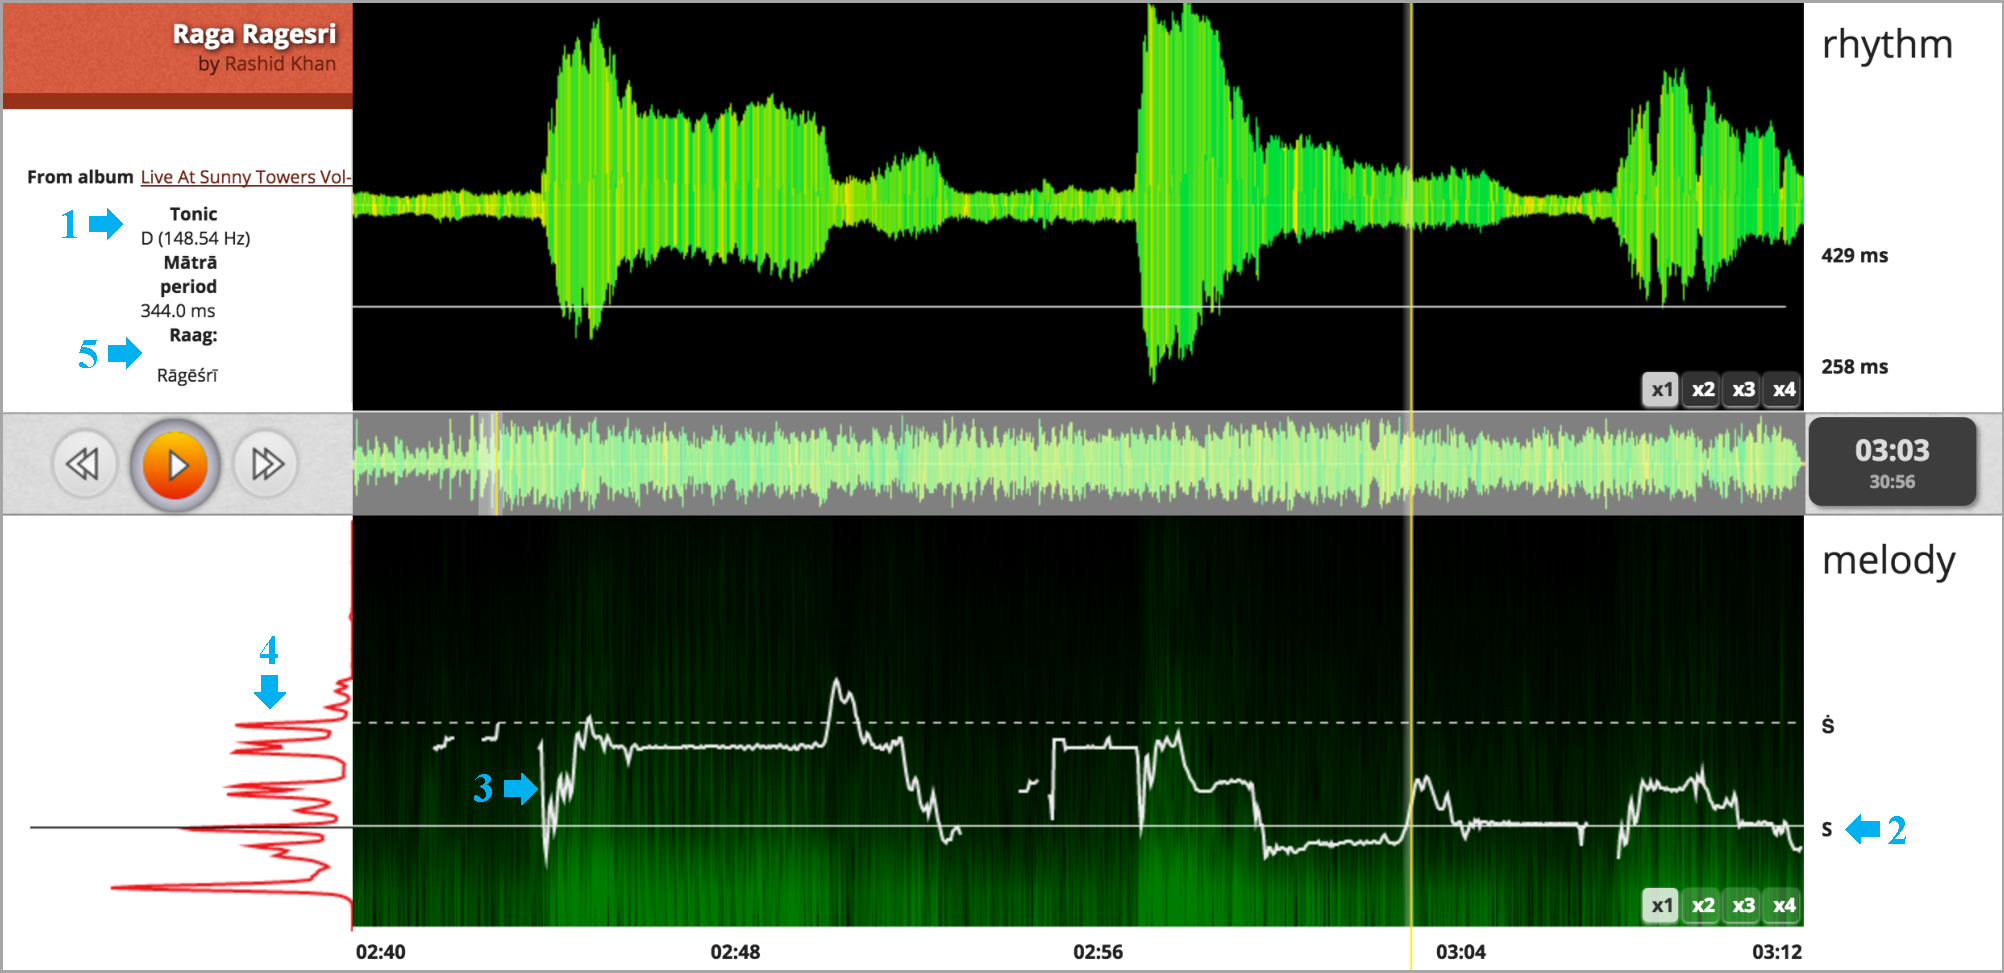
\includegraphics[width=\figSizeHundred]{ch08_applications/figures/dunyaScreenshot.pdf}
		\end{center}
		\caption{Screenshot of the recording page in Dunya showing extracted music descriptors and associated metadata}
		\label{fig:dunya_recording}
\end{sidewaysfigure}

While the Web interface provides an easy and a quick access to the data, for a more comprehensive access mainly meant for researchers and developers Dunya provides a restful \gls{api}. Through the \gls{api} it exposes audio recordings, gathered metadata and extracted music descriptors. it can be used by researchers to create different datasets from the CompMusic corpora. To further facilitate the usage of this \gls{api}, its Python\footnote{\url{https://www.python.org/}} wrapper, \gls{pycompmusic}\footnote{\url{https://github.com/MTG/pycompmusic}}, is provided. Using this tool with just a few lines of code the entire corpora and associated metadata can be retrieved. An example usage of \gls{pycompmusic} is shown below.

%\lstset{language=Python,
%	numbers=left,                    % where to put the line-numbers; possible values are (none, left, right)
%	numbersep=5pt,
%	basicstyle=\footnotesize,
%	numberstyle=\tiny,
%	frame=tb,
%	columns=fullflexible,
%	showstringspaces=false
%	}
%
%\begin{lstlisting}[frame=bt] 
%from compmusic import dunya as dn
%from compmusic.dunya import carnatic as ca										
%
%dn.set_token("60312f59428916bb854adaa208f55eb35c3f2f07")		#authorization
%
%recs = ca.get_concerts()																	  #Fetching all the concerts
%
%len(recs)
%
%\end{lstlisting}

\begin{verbatim}
In [1]: from compmusic import dunya as dn
In [2]: from compmusic.dunya import carnatic as ca
In [3]: dn.set_token("<dunya api token>")
In [4]: concerts = ca.get_concerts()
In [5]: len(concerts)
Out[5]: 328
In [6]: concerts[1]
Out[6]: 
       {u'mbid': u'c5d9d3bd-bc01-4104-b874-d55219bd0e54',
        u'title': u'Madrasil Margazhi 2006'}
In [7]: recs = ca.get_recordings()
In [8]: len(recs)
Out[8]: 3533
In [9]: recs[1]
Out[9]: 
       {u'mbid': u'01f863b7-46b4-44f5-b547-fcbaa1f66348',
        u'title': u'Vetta Veli'}        
\end{verbatim}
\TODO{make this paragraph better}
This is an example of querying metadata for Carnatic music collection\footnote{\url{https://musicbrainz.org/collection/55412ad8-1b15-44d5-8dc8-9c3cb0cf9e5d}} of the CompMusic Corpora. After importing relevant modules (ln~[1] and [2]), the first step is user authentication, which requires a Dunya \gls{api} token (ln~[3]). This token can be obtained by registering in to Dunya. We obtain a list of all 328 concerts in Carnatic collection (ln~[4]), where information about each concert is contained in a dictionary (Out~[6]). Subsequently, we also present a query to obtain a list of all 3533 recordings in the collection (ln~[7]) and show the structure of the response (Out~[9]). Using the \acrshortpl{mbid} of the concerts and the recordings we can obtain more information about those entities. The Dunya \gls{api} provides access to the editorial metadata, the audio recordings and the extracted audio features for all the music collections in the CompMusic corpora.

\section{Mobile Applications: Sar\={a}ga and Riy\={a}z}
\label{sec:mobile_apps_camut}

\gls{saraga} and \gls{riyaz} are the two mobile applications developed as a part of the \gls{camut}\footnote{\url{http://mtg.upf.edu/projects/camut}} project, which aims to explore the commercial exploitation of the technologies developed in the CompMusic project. These applications aim to foster learning, teaching and appreciation of Indian music forms. Both these applications incorporate parts of the outcome of our research work presented in this thesis. We provide below a brief description of these applications. 

\subsubsection{Sar\={a}ga}
\label{sec:saraga}

\begin{figure}
	\centering
	\begin{subfigure}[b]{0.48\textwidth}
		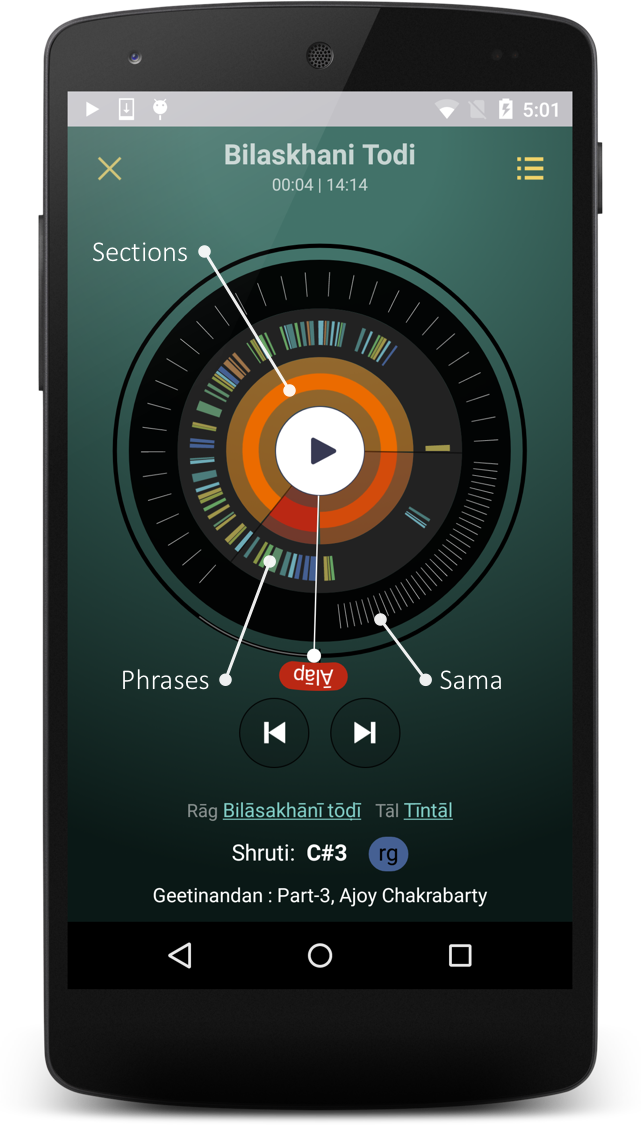
\includegraphics[width=\figSizeNinety]{ch08_applications/figures/saraga1.png}
		\caption{Full music piece}
		\label{fig:saraga_full_piece}
	\end{subfigure}
	\begin{subfigure}[b]{0.48\textwidth}
		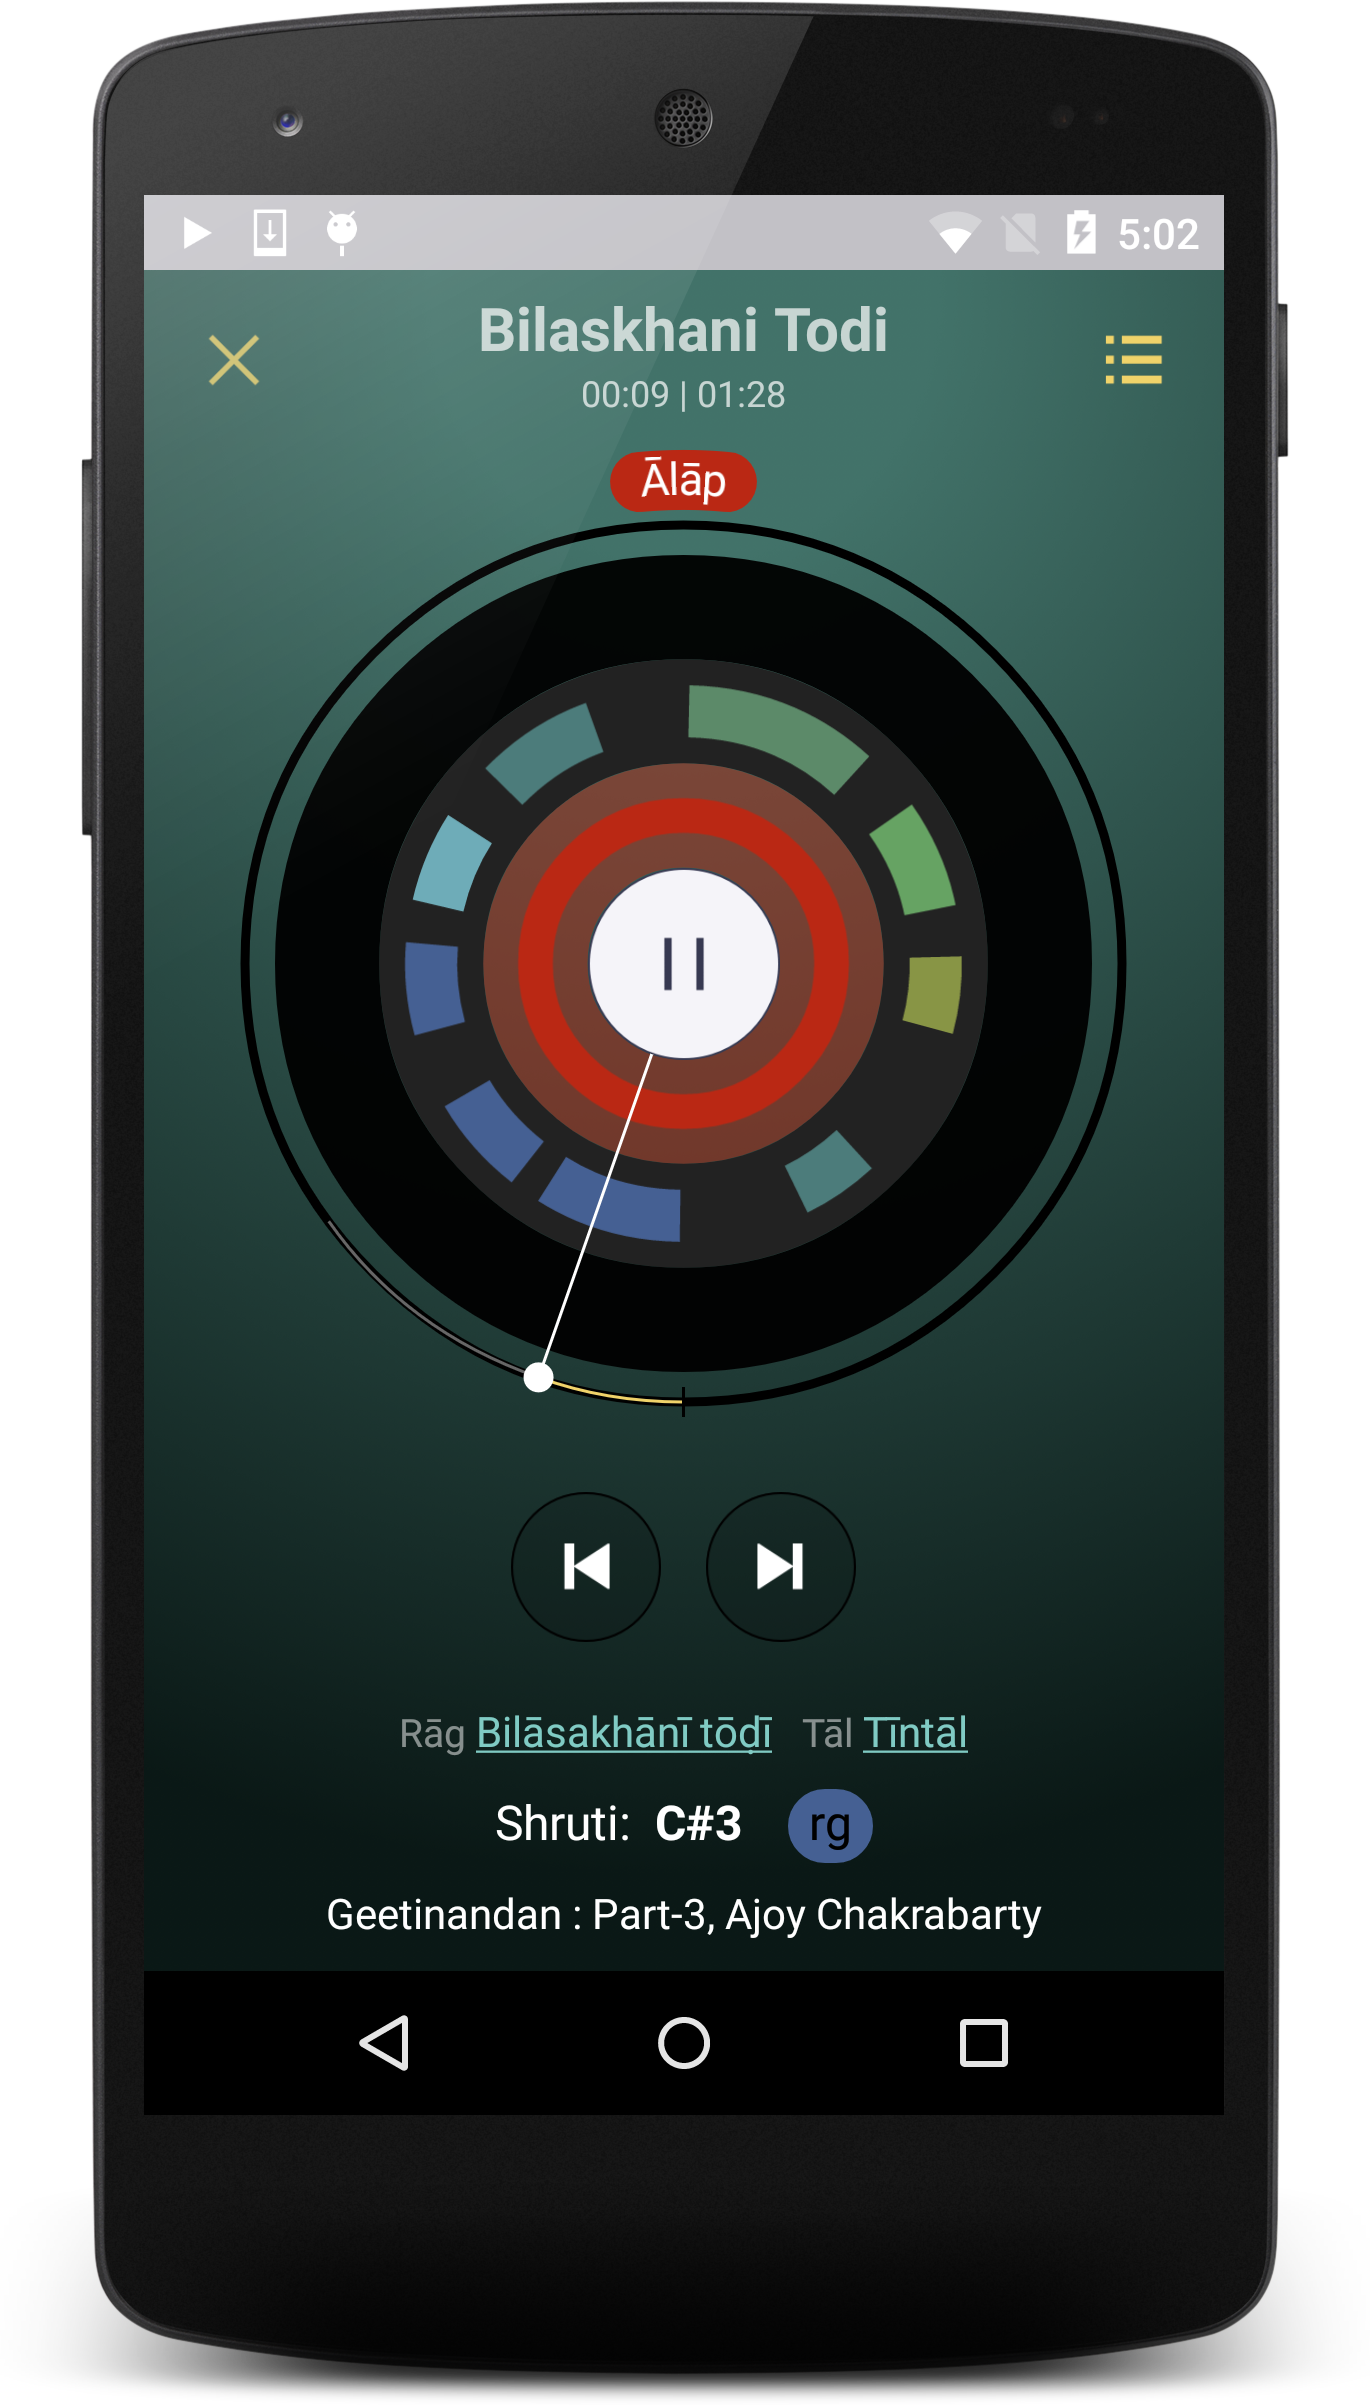
\includegraphics[width=\figSizeNinety]{ch08_applications/figures/saraga2.png}
		\caption{\Gls{alap} section (zoomed in)}
		\label{fig:saraga_alap_section}
	\end{subfigure}
	\caption{Screenshots of Sar\={a}ga mobile application showing a music piece of Hindustani music. (a) shows the entire music piece, (b) shows the \gls{alap} section in the piece. Melodic phrases are marked by the colored arches. Tonic (\gls{shruti}) of the recording is shown at the bottom along with the current playing melodic phrase.}
	\label{fig:saraga_screens}
\end{figure}

\Gls{saraga} is a mobile application that provides an enriched listening atmosphere over a collection of Carnatic and Hindustani music that is released under Creative Commons license\footnote{\url{https://creativecommons.org/}}. It is meant for music connoisseurs and students of these art music traditions to navigate, discover and listen the music using culturally relevant concepts. \gls{saraga} contains inclusive designing of innovative visualizations and inter and intra-song navigation interfaces that present musically rich information to the user in a compact way. The time synchronized visualizations of musically relevant facets such as melodic patterns, \gls{sama} locations and sections provides a user with better understanding and appreciation of these music traditions.

In~\figref{fig:saraga_screens} we show a screenshot of the recording page of in \gls{saraga} playing a music piece\footnote{\url{https://musicbrainz.org/recording/3124479b-5118-4cf3-823f-8fefad45e586}} in Hindustani music. In~\figref{fig:saraga_screens}\,(a) the entire music piece is visualized. Information regarding the sections, melodic patterns and the \gls{sama} locations is displayed through the concentric circles as indicated in the screenshot. As the playback advances in time along the circle, these descriptors are highlighted based on the current time. For example, in~\figref{fig:saraga_screens}\,(a) the melodic phrase ``rg'' is being sung in the piece, which is highlighted at the bottom of the screen. Since the music performances in \gls{iam} can last long (sometimes up to an hour), \gls{saraga} interface allows to tap and zoom into a particular section. An example of this is shown in~\figref{fig:saraga_screens}\,(b) wherein the \gls{alap} section is selected. Furthermore, a user can also tap on a particular melodic pattern to then go to a new page where all the occurrences of that pattern in the recording are shown together. These functionalities facilitate a user to better understand the structuring of different musical facets in a piece of \gls{iam}. In addition to these descriptors there is accompanying data shown at the top and the bottom of the screen, which includes editorial metadata and \gls{shruti} (tonic) information. The text strings corresponding to the musical concepts (\gls{raga} and \gls{tala}) are hyper-linked to their respective pages, where that musical concept is described using a set of representative audio examples. 


\subsubsection{Riy\={a}z}
\label{sec:riyaz}

\begin{figure}
	\begin{subfigure}{\textwidth}
			\centering
		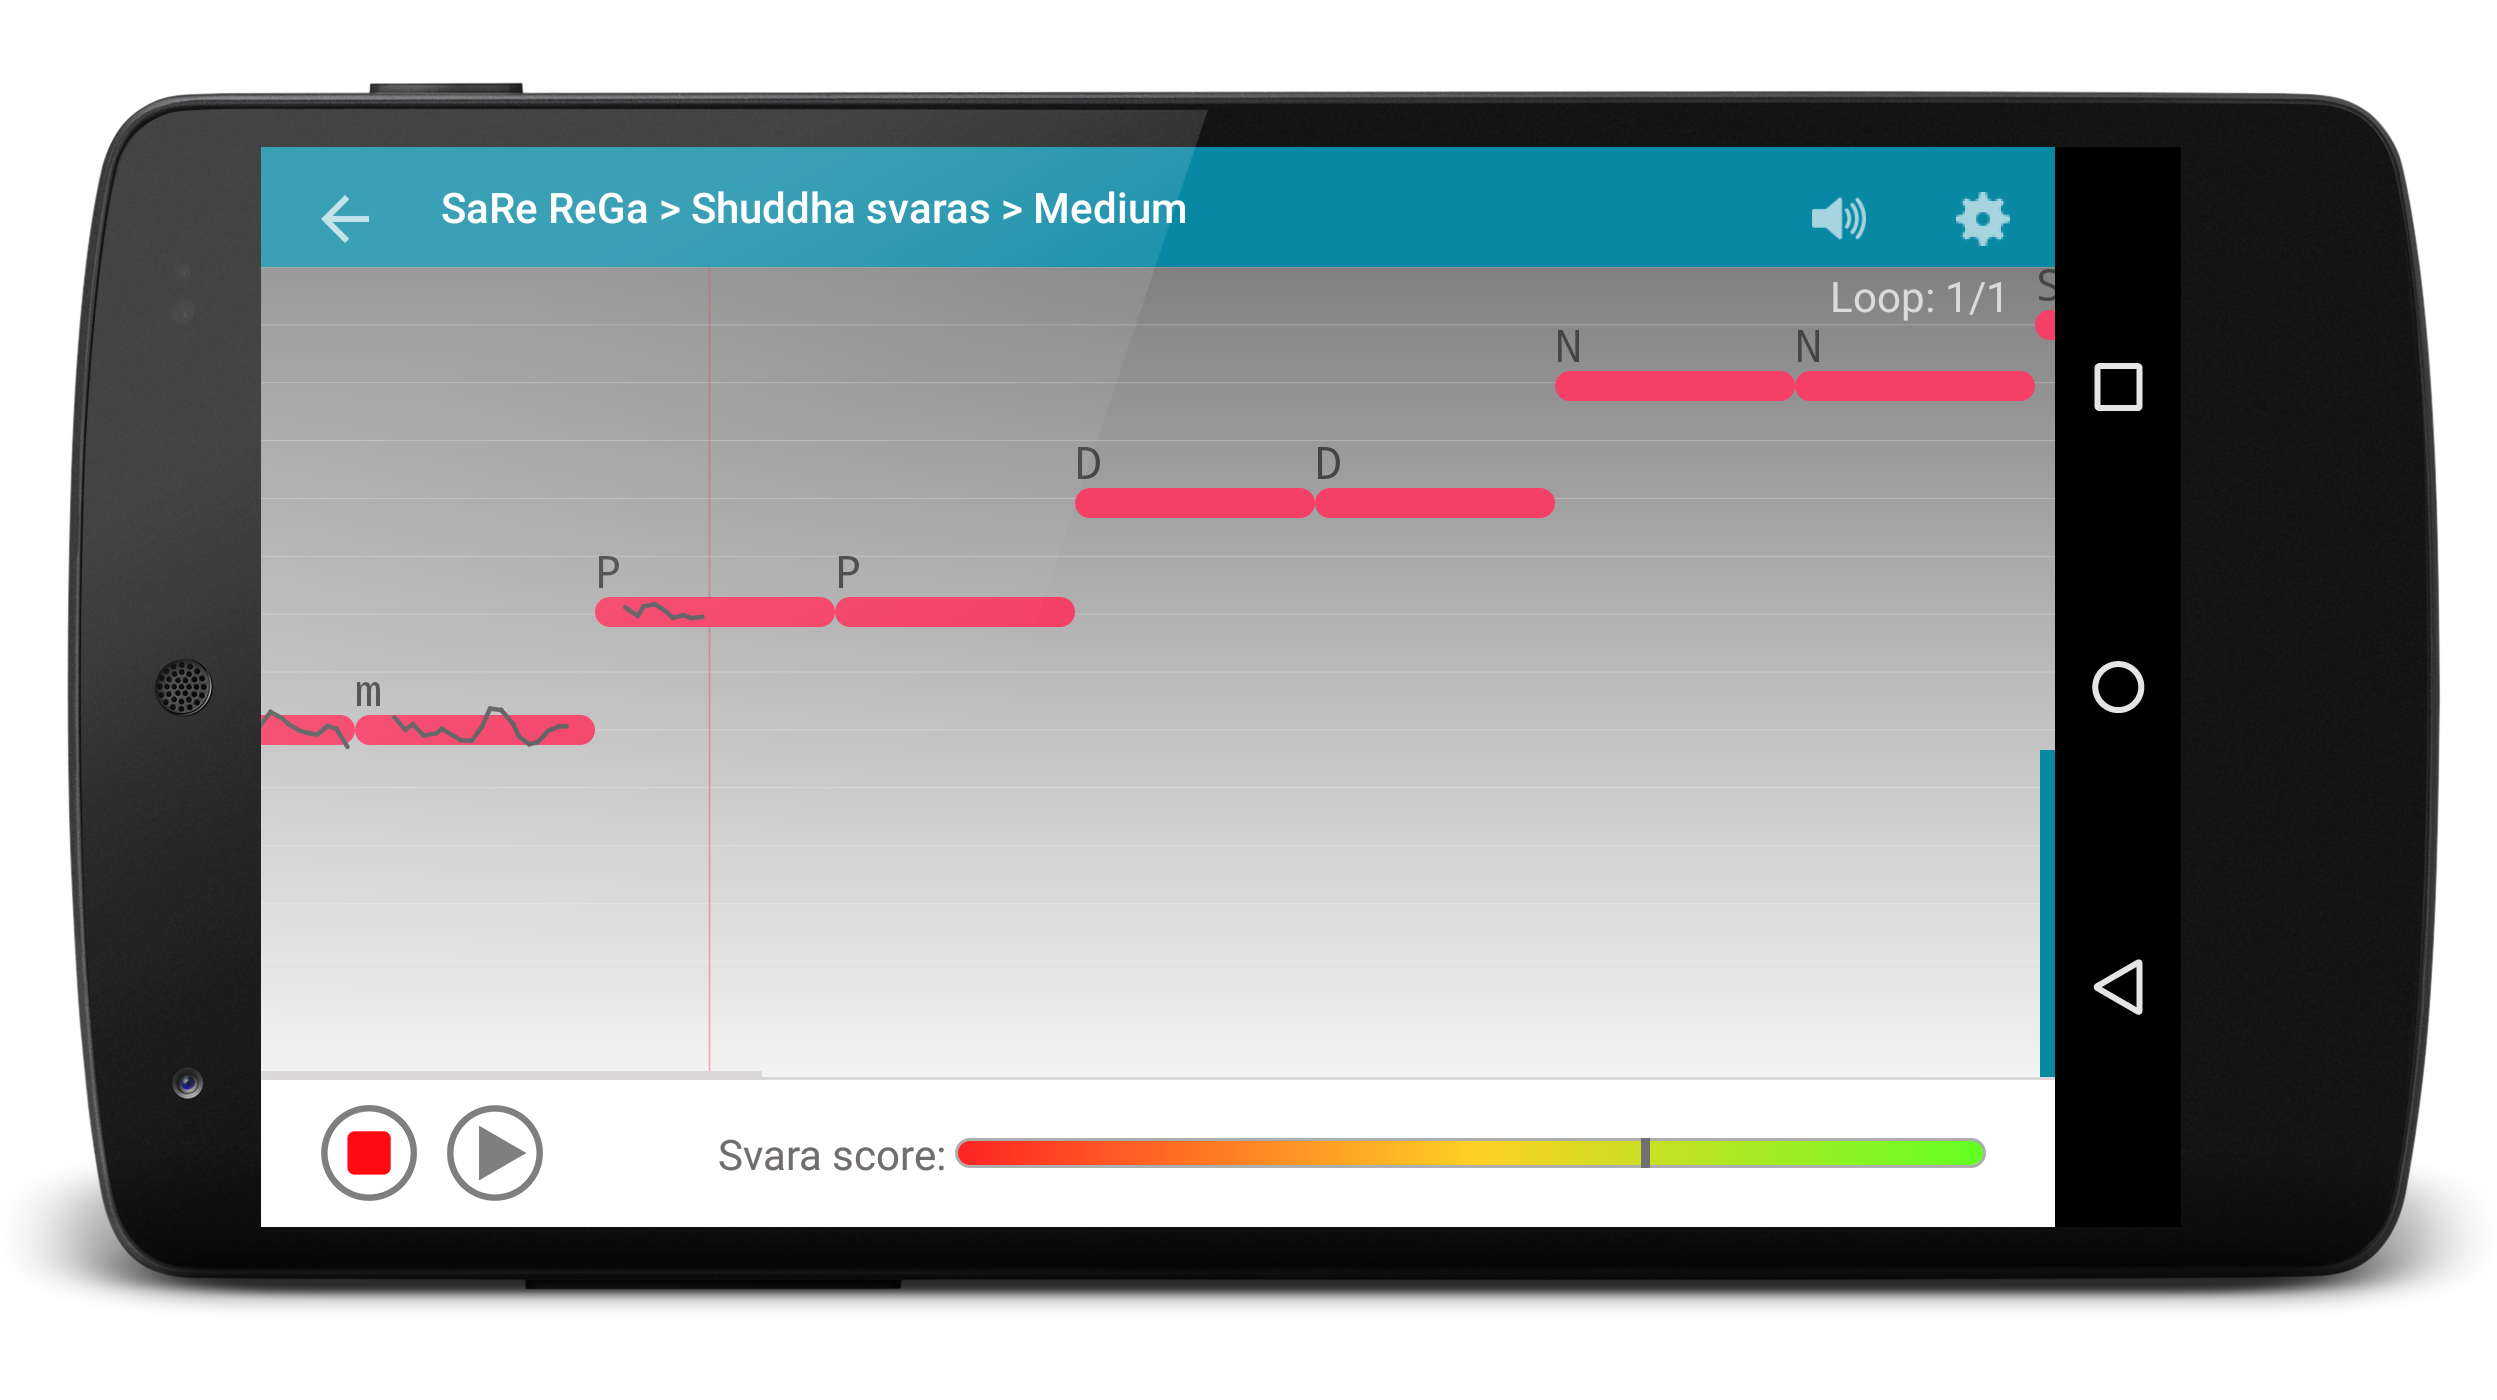
\includegraphics[width=\figSizeSeventy]{ch08_applications/figures/riyaz1.png}
		\caption{Evaluation screen}
		\label{fig:riyaz_evaluation_screen}
	\end{subfigure}
	\begin{subfigure}{\textwidth}
			\centering
		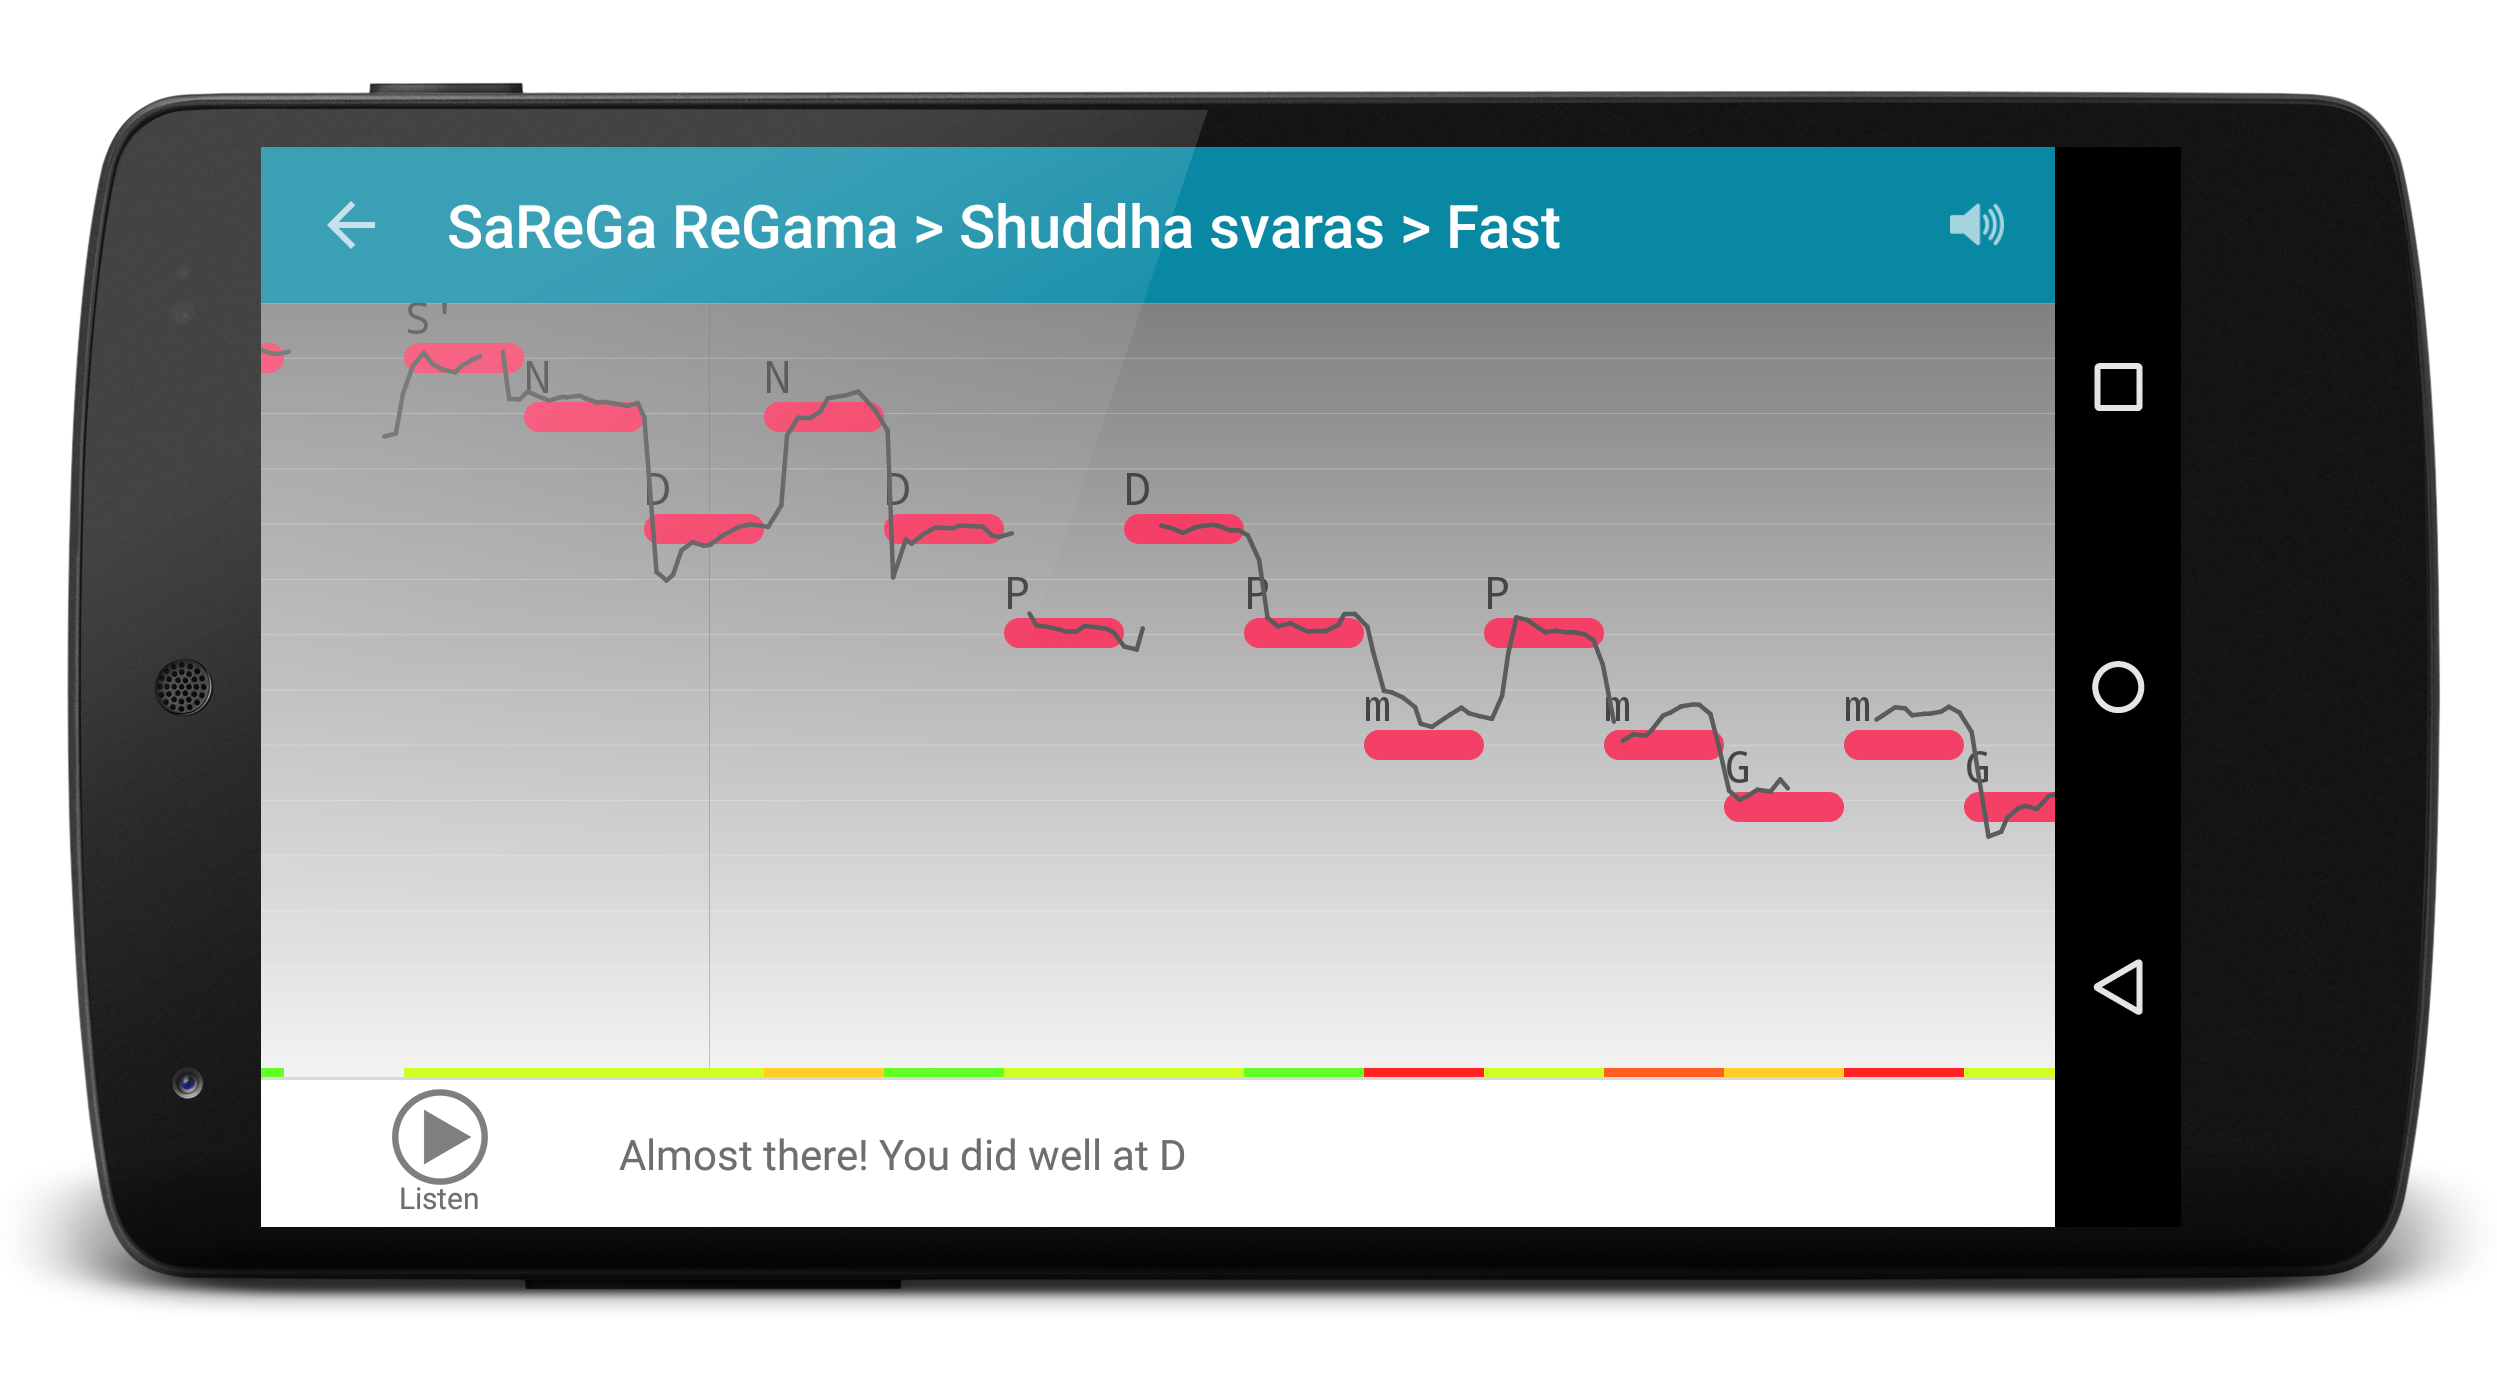
\includegraphics[width=\figSizeSeventy]{ch08_applications/figures/riyaz2.png}
		\caption{Feedback screen}
		\label{fig:riyaz_feedback_screen}
	\end{subfigure}
	\caption{Screenshots of the Riy\={a}z (Beta) mobile application}
	\label{fig:riyaz_screens}
\end{figure}

\gls{riyaz} is a mobile application that aims to facilitate music learning for beginner to intermediate level music students of \gls{iam} by making their practice sessions more efficient. It does it by simulating a classroom environment in which the learning happens through imitating the musical exercises build by processional musicians. The application performs singing assessment and provides a detailed feedback, wherein it highlights the mistakes and gives suggestions to improve. In~\figref{fig:riyaz_screens}\,(a) we show the main evaluation screen of \gls{riyaz} where a user can visualize in real-time the pitch track and \gls{svara} score. Post practice session, a detailed feedback is provided as shown in~\figref{fig:riyaz_screens}\,(b).  Note that \gls{riyaz} is a work in progress with a prototype version already available at the time of writing this thesis. Currently there are 1000+ users with 15000+ user sessions. 


\section{Demos}
\label{sec:demos}

We now proceed to present two prototype Web-based applications that demonstrate the outcome of our pattern discovery approach. In addition, we also present \gls{ragawise}, a prototype Web application for real-time \gls{raga} recognition. 

\subsection*{Demo1: Melodic Patten Discovery}

One of the motivations behind pattern discovery is to explore novel relationships in the data and extract new knowledge. However, it is a challenging task to evaluate these aspects  in a quantitative evaluation setup, wherein available ground-truth (typically comprising expert annotations) is used as a basis to measure the quality of the output. It becomes even more challenging when such analyses are performed on large datasets such as the case with ours, in which obtaining a ground-truth becomes practically unfeasible.  In the study presented in~\secref{}, we performed melodic pattern discover in audio collections of Carnatic music comprising nearly 365\,hours of music. Though we performed a quantitative evaluation using a randomly sampled subset of the output, the evaluation numbers do not convey much in terms of the musical novelty of the patterns. 

In order to facilitate informal evaluations, take feedback from musicians, identify novel outcomes, and eventually, to improve the quality of the output of our pattern discovery methods we built two Web-based application that exposes the resultant patterns. 

\begin{figure}
	\begin{center}
		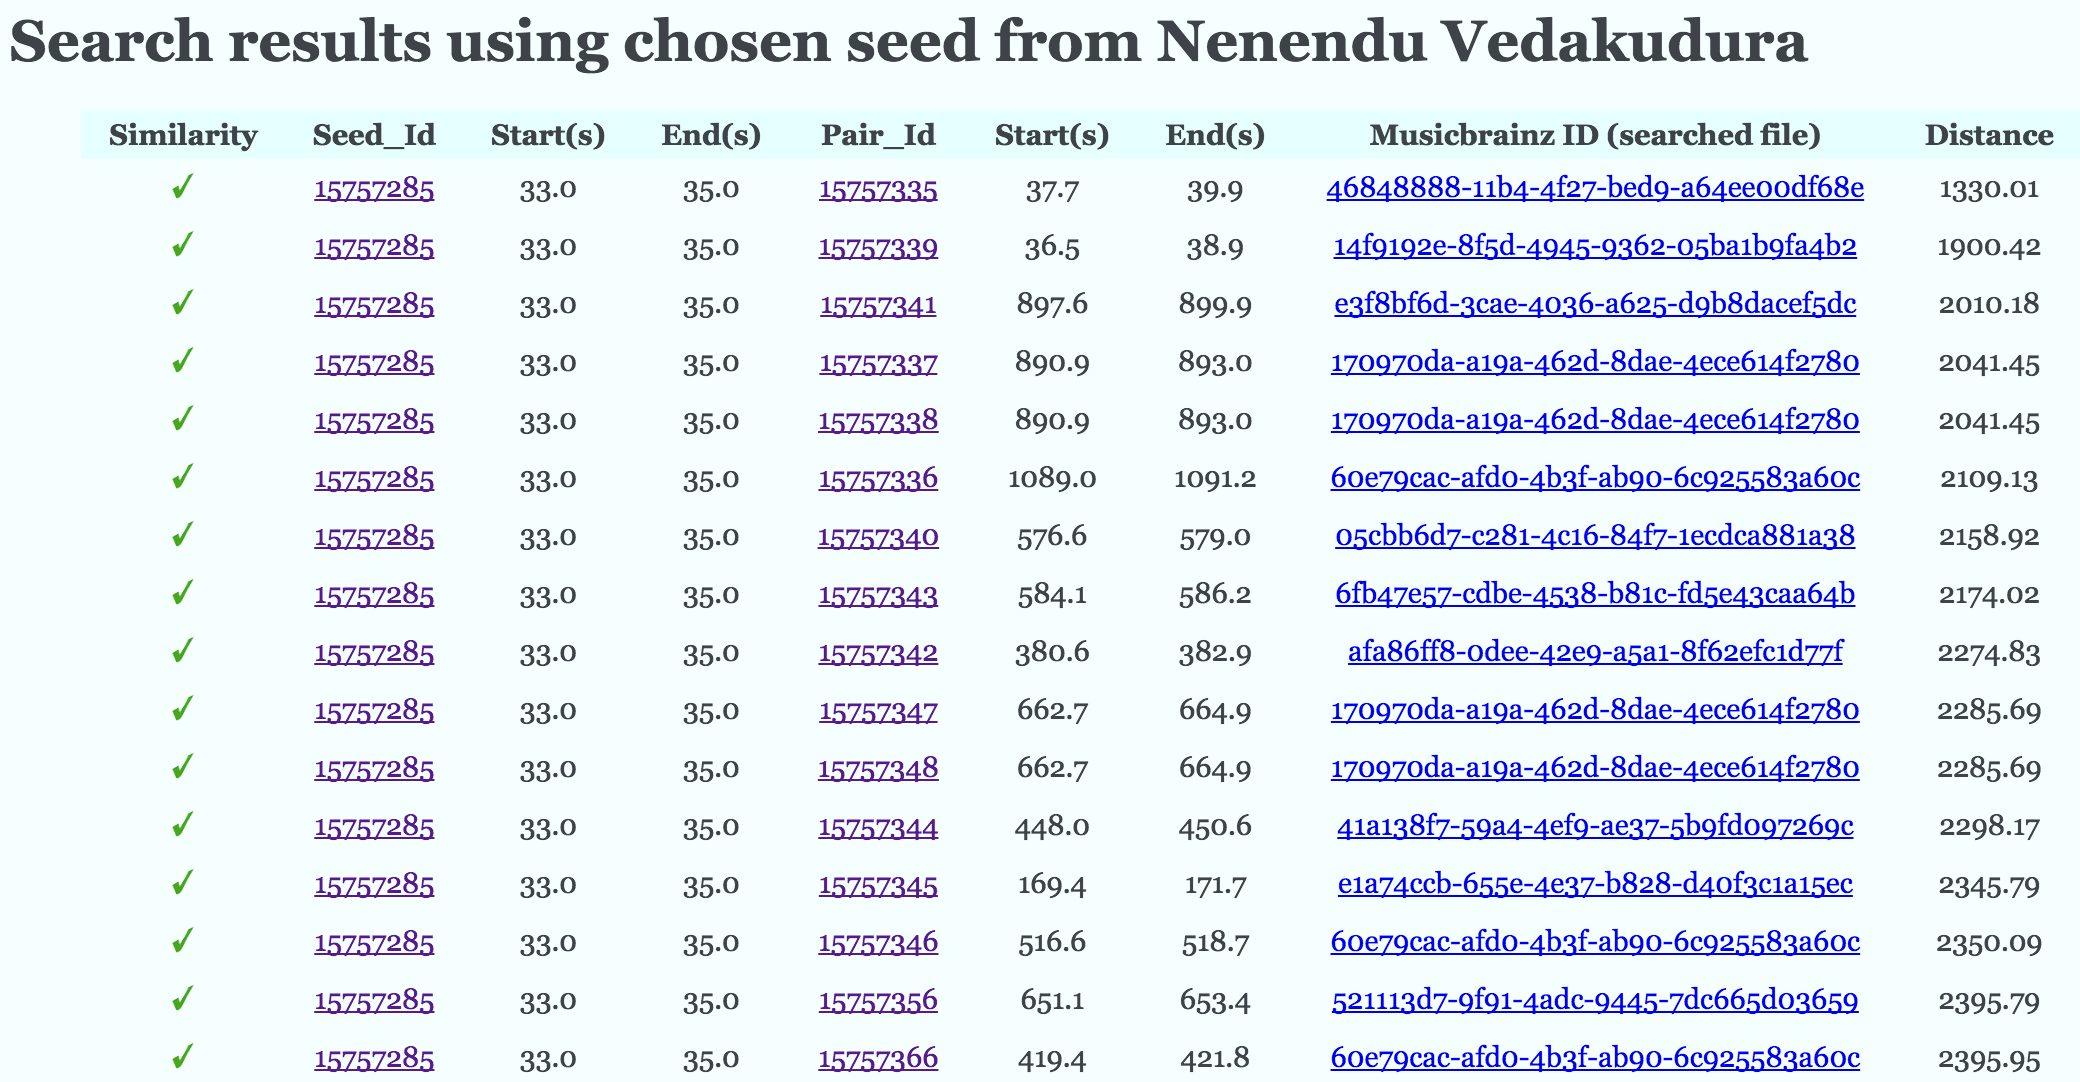
\includegraphics[width=\figSizeHundred]{ch08_applications/figures/patternBrowsing1.png}
	\end{center}
	\caption{Screenshot of a Web demo for navigating through the discovered melodic patterns organized by artists, releases and recordings.}
	\label{fig:browser_patterns}
\end{figure}

Our first demo application allows to browse through all the melodic patterns discovered in the study reported in~\secref{}. Since determining a meaningful similarity threshold is in itself a challenging task, we selected a fixed number of closest pattern matches in the output. To recall, 25 closest seed pattern pairs were selected within a recording, and for each seed pattern its 200 closest neighboring patterns were selected  across the entire music collection. This resulted in around 15\,million patterns for our audio collection that comprise 1764\,recordings. This demo allows us to navigate through all the recordings in the collection, fetch all the seed patterns for a recording, and for each seed pattern, fetch their closest patterns from the entire music collection. In~\figref{fig:browser_patterns}, we show a screenshot of a page where a list of closest melodic patterns for a seed pattern is displayed. All the listed melodic patterns can be played and listened to. We notice that the retrieved patterns are from different recordings bearing different \glspl{mbid}. These recordings are from different artists with different tonic pitches, and even across vocal and instrumental music. 

\begin{figure}
	\begin{center}
		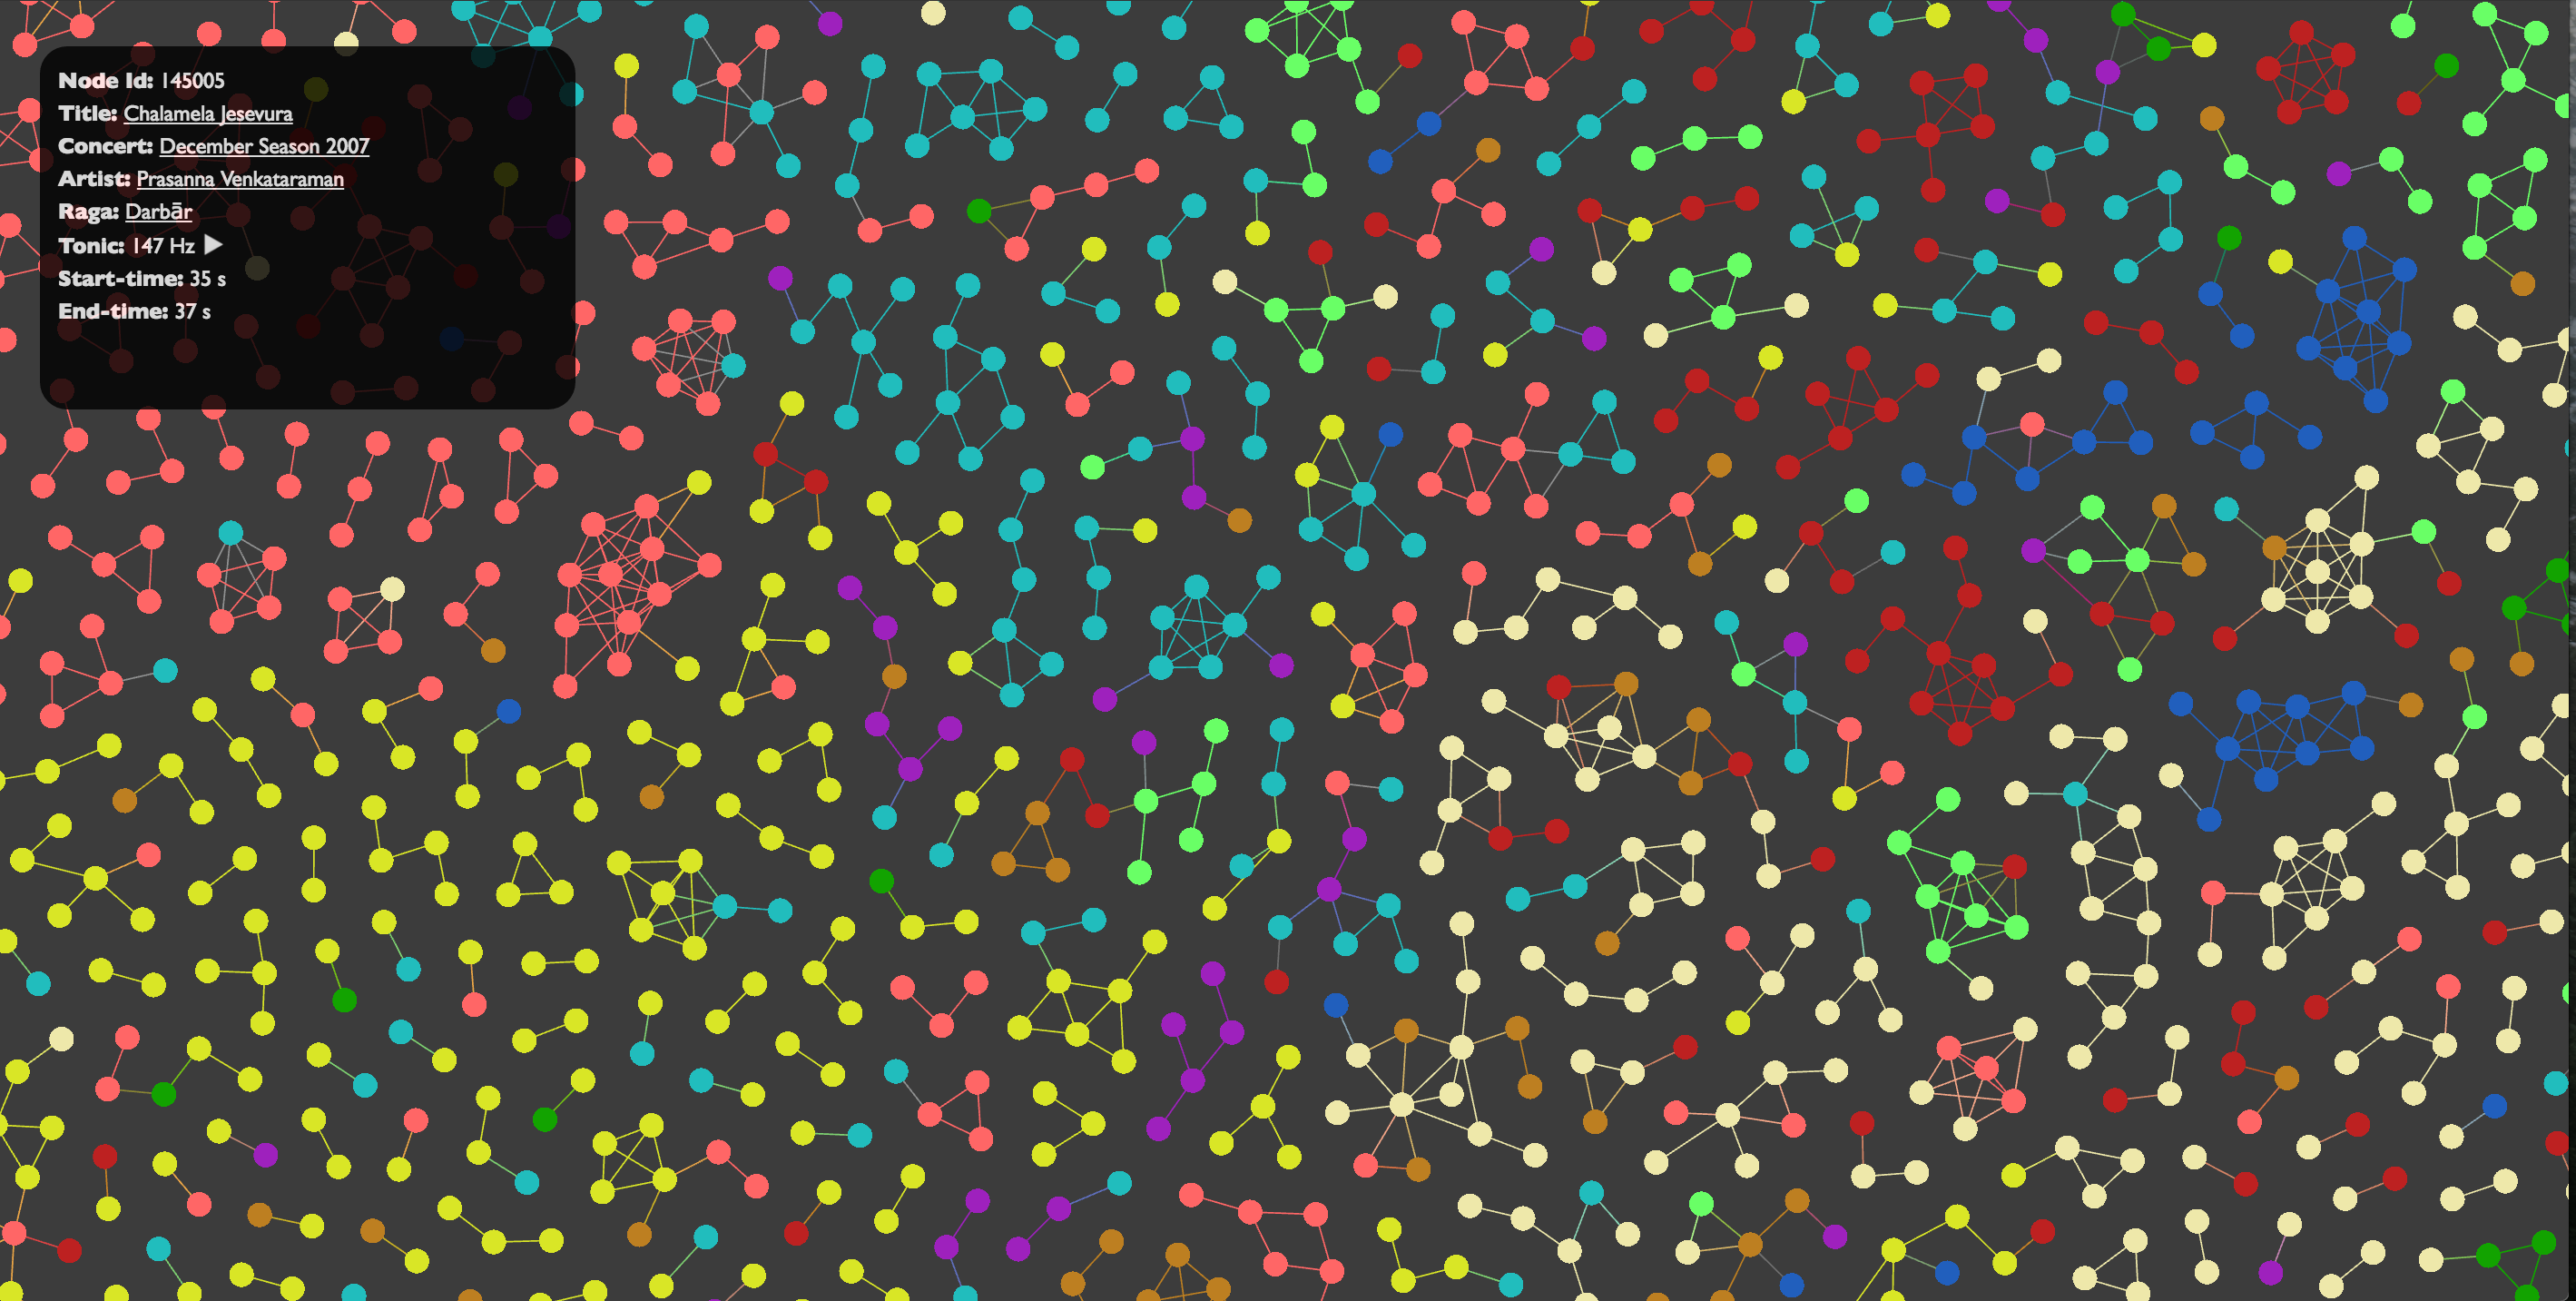
\includegraphics[width=\figSizeHundred]{ch08_applications/figures/patternNetwork1.png}
	\end{center}
	\caption{Screenshot of a Web demo of a network of the discovered melodic patterns. Colors indicate different \glspl{raga}.}
	\label{fig:network_patterns}
\end{figure}

The demo described above presents melodic patterns structured in an hierarchical way, which is useful when the reader is curious to look for patterns in a particular music piece or by a particular artist. An alternate way to present these patterns is through an interlinked network of them. Such a network visualization makes it easier to identify interesting and novel relationships between different music pieces, artists, and sometimes, even across \glspl{raga}. In~\figref{fig:network_patterns} we show a screenshot of our second demo that presents a network visualization of discovered melodic patterns. These melodic patterns are ones obtained in the study described in~\secref{}. Note that in this study we employed a network analysis to also determine a melodic similarity threshold, as a result of that filtering we retain only the musically meaningful connections between the melodic patterns. The nodes of the network are the melodic patterns and the edges represent a binary melodic similarity between the nodes.  In addition, for each node we also provide the accompanying information of the audio recording from which it is extracted (\figref{fig:network_patterns}, top-left corner). Furthermore, we also provide an option to play a tone that corresponds to the tonic of the recording. This helps to establish the tonal context of the melodic pattern.

Both the Web demos described above provide useful insights into the outcome of our approaches. They are made available online (\appref{sec:resources}). 


\subsection*{Ragawise: Realtime Raga Recognition}
\label{sec:ragawise}

In~\chapref{} we described our computational approaches for \gls{raga} recognition in detail. Our objective was to develop novel methods to obtain a \gls{raga} label for a recorded music performance. As mentioned earlier, there are several applications of these methods such as automatic \gls{raga} annotation of large audio archives, \gls{raga}-based music retrieval, establishing meaningful similarity measures across recordings and music pedagogy. In this section we present a prototype Web application, \gls{ragawise}, which demonstrates the usability of such systems in the context of music pedagogy. 

\gls{ragawise} is a real-time \gls{raga} recognition prototype system~\citep{ragawise}. It uses \gls{pcp}, pitch transitions and melodic patterns to recognize \gls{raga} from an incoming audio stream. For each \gls{raga} it stores a dictionary of the \glspl{svara}, \gls{svara} transitions, and typical melodic patterns. It processes the input vocals in real-time to estimate pitch, and subsequently performs melody transcription. The likelihood of each \gls{raga} is updated in real-time based on the identified of \gls{raga} elements in the melody. In order to highlight the melodic events that are characteristic of a \gls{raga}, a dynamic visualization of the evolution of the likelihood of all the \glspl{raga} is performed. We present a screenshot of \gls{ragawise} in~\figref{fig:ragawise}, where different panels are marked by blue arrows. In the top panel (arrow~1) we display the transcribed melody symbols (\glspl{svara} in this case) using the pitch track obtained in real-time (arrow~2). We continuously process the transcribed melody to detect the presence of different melodic elements, and once detected, we highlight the associated \glspl{raga} (arrow~3,4,5). We also compute a cumulative salience score of each \gls{raga} based on the frequency of the detected melodic elements (arrow~6). \TODO{make this para better}

Note that \gls{ragawise} is a team effort, made a part of the hackday, HAMR, in ISMIR-2015. It is done in collaboration with Kaustuv Kanti Ganguli, Swapnil Gupta and Ajay Srinivasamurthy. 

%\TODO{I just wrote something in a hurry, discuss with Kaustuv if its worth putting such apoint, and also if he would like to make it sound better}
%There are different sets of \glspl{raga} that share common melodic elements. For example, there are \glspl{raga} that share set of \glspl{svara}, while some others may have similar melodic phrases. In a \gls{raga} rendition an important aspect is to understand when to bring in characteristic melodic elements of a raga and when to use elements which are also used in similar ragas. This aspect is used to control the musical tension, wherein an artist gives away clear cues for a particualr raga after he has built the tension. In ragawise we not just identify the closest possibility of a raga but also update the saliences of all the ragas based on the sung melody. Such a system can be used by teachers to demonstrate characteristics aspects of ragas and the ones which are shared amongst different ragas. Also for a student it is helpful to observe if unknowingly he is using some elements of another raga.

\begin{sidewaysfigure}
	\begin{center}
		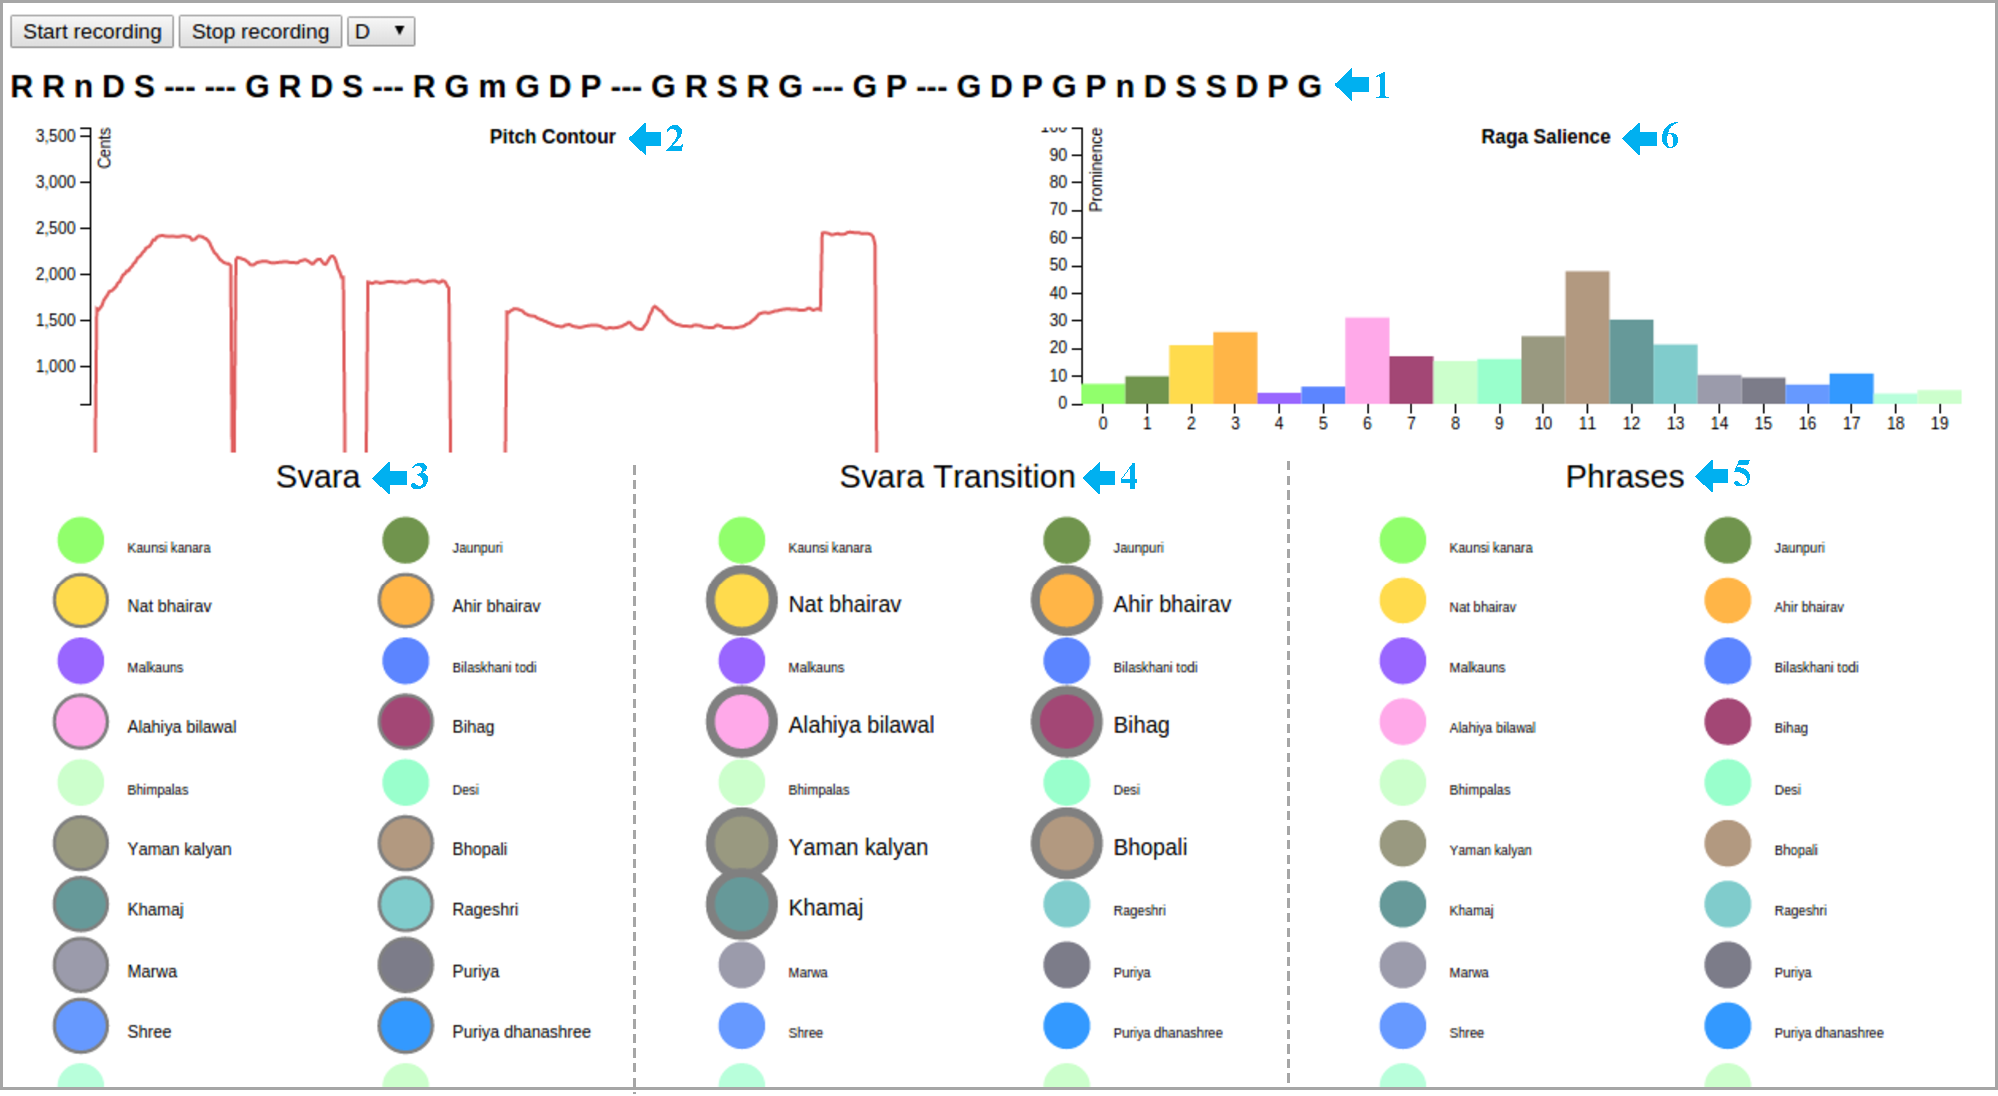
\includegraphics[width=\figSizeHundred]{ch08_applications/figures/ragawise.pdf}
	\end{center}
	\caption{Screenshot of \gls{ragawise}, which illustrates real-time pitch tracking, melody transcription and \gls{raga} salience evolution. Bottom panel shows a list of \glspl{raga} for each melodic element (\gls{svara}, \gls{svara} transition and melodic patterns). \Glspl{raga} for which a particular melodic element is detected in the audio stream are highlighted.}
	\label{fig:ragawise}
\end{sidewaysfigure}

\TODO{Please add musicological wala kaam yaar!}
%
%\section{Tools for Musicological Studies}
%\COMMENT{Write this section if you get time at the end}

\section{Summary}
\label{sec:applications_summary}

In this section we presented a few examples of concrete applications that utilize the output of the work presented in this thesis. We presented Dunya, which comprise all the data and software tools developed in the CompMusic project. We briefly described ways to access different types of data within the CompMusic corpora. A number of datasets can be created to study different aspects of \gls{iam} using these corpora and tools. Subsequently, we presented three demos that being forward the outcome of our approaches. They provide useful insights, which can be looped back to further improve our systems. We also presented two mobile applications that demonstrate the utility of our work in the context of commercial applications. These applications give an idea about the context in which our work is usable. Overall, we see that our work is useful in several ways, in different contexts and, there can be a number of interesting applications built on top of it. 



